\section{Requests}
\label{sec:requests}

Considering a harbour crane represented in Figure \ref{fig:harbour-crane}, the requests for `Assignment 2' are the followings:

\begin{itemize}
    \item Define a FE model of the structure in the 0-8 Hz frequency range considering a safety factor equal to 2.
    \item Calculate the structure's natural frequencies and vibration modes up to the 3rd mode. Plot the mode shapes with the indication of the associated natural frequencies.
    \item Calculate the structure frequency response functions which relate the input force applied at position A in vertical direction to the outputs vertical displacement at point A and horizontal displacement at point B. Assume the input force to vary in the 0-8 Hz frequency range and set the frequency resolution to 0.01 Hz.
    \item Using the modal superposition approach and considering the structure's first two modes, calculate the frequency response functions which relate the same input force of question 3 (vertical force applied in node A) to the horizontal displacement of node B. Plot the corresponding magnitude and phase diagrams superimposed to those obtained in item 3. Point out the differences and comment the results.
    \item Calculate the structure frequency response function relating the input force applied at position C in vertical direction to the output axial force in the right column evaluated at point O2. Assume the input force to vary in the 0-8 Hz frequency range and set the frequency resolution to 0.01 Hz.
    \item Compute the static response of the structure due to the weight of the entire structure. Plot the deformed shape of the structure compared to the undeformed configuration and compute the value of the maximum deflection.
    \item Optional - Calculate the vertical displacement time history of point A, taking into account a moving load traveling between points D and A. The load begins with zero initial velocity, uniformly accelerates over the first 8 meters, keeps a constant velocity over the next 8 meters and then decelerates until reaching point A with null velocity. Total time to travel from D to A is 20s.
\end{itemize}

\begin{figure}[H]
    \centering
    \scalebox{-1}[1]{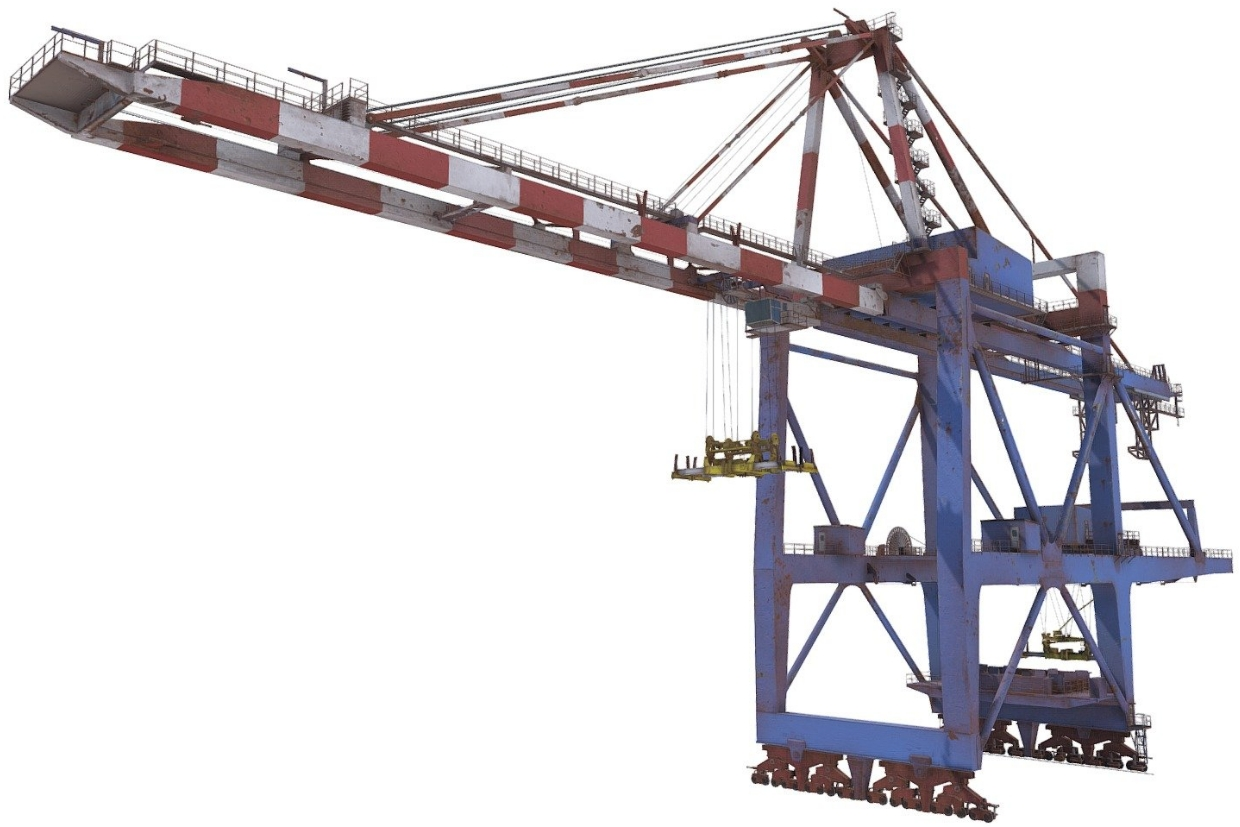
\includegraphics[width=0.7\textwidth]{img/harbour-crane-image.jpeg}}
    \caption{Harbour crane}
    \label{fig:harbour-crane}
\end{figure}